\chapter{One-dimensional reservoir case}

For simple understanding and working out the application of the methods, first, an abstract one-dimensional reservoir case is presented in this chapter. The underlying model and basic approach are inherited from \citet{delaVarga2016}. Parameters were adapted to more appropriately represent a reasonable geological petroleum system, consisting of a reservoir with overlying seal in the subsurface. In doing this, a certain economic significance is ascribed to the model and further relevant questions can be derived. Regarding the petroleum sector, the problem of interest is most commonly one of estimating the volume of resources or monetary value contained in an oil or gas reservoir. Limiting the model to only one dimension and a small number of uncertain parameters allows for a relatively straightforward and simplified approach to assessing an abstract type of value for a reservoir and designing a respective loss function for value estimation. A step by step derivation of such as case follows below.

	\section{Constructing the one-dimensional model}\label{sec:1D_construction}
	
	\citet{delaVarga2016} constructed a simple geological model using three uncertain positions in vertical one-dimensional space, marking hypothetical boundaries of layers in a subsurface column. The location probabilities for these points are defined by sampling from normal distributions. Standard deviations of these distributions increase with depth, representing an increase in uncertainty. For an approximate representation of a petroleum system, the distribution means were set to depths of 2000 m (seal top), 2050 m (reservoir top) and 2200 m (reservoir bottom). These points confine two layers in the middle, from which the upper one can be labeled as seal and the lower one as reservoir. The resulting model with its possible layer boundary locations is illustrated in Figure \ref{fig:1D_model}.
	
	\begin{figure}[h]
		\centering
		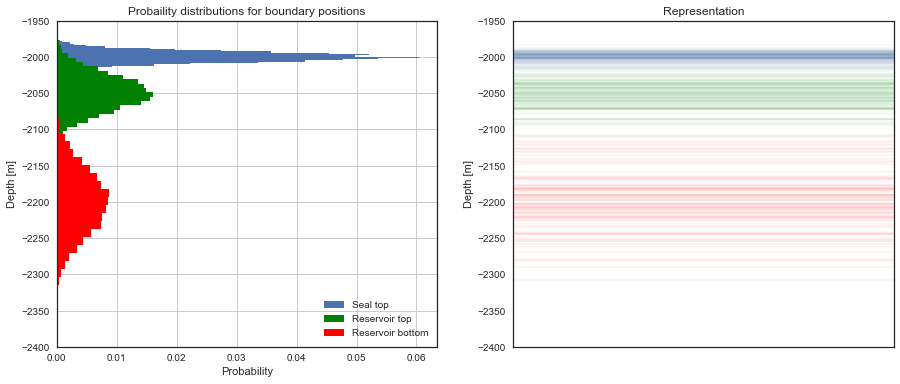
\includegraphics[width=1\textwidth]{Figures/1D_model.png}
		\caption{Probability distributions for positions of layer boundaries in the subsurface and a respective representation using lines.}\label{fig:1D_model}
	\end{figure}
	
	\section{Assessing reservoir quality using scores}\label{sec:scoring}
	
	The next step is to find a way to assess the quality of the reservoir from a petroleum industry perspective in such a simplified model. What can be deduced from the distributions of layer boundary locations, is the thickness of the seal and the reservoir, as well as the depth of both, again as probability distributions. To assess the reservoir quality in an abstract way, it can be assigned a score. This score is made dependent on the three uncertain parameters (1) reservoir thickness, (2) reservoir top depth and (3) seal thickness (see Figure \ref{fig:3_parameters}).
	
	\begin{figure}[h]
		\centering
		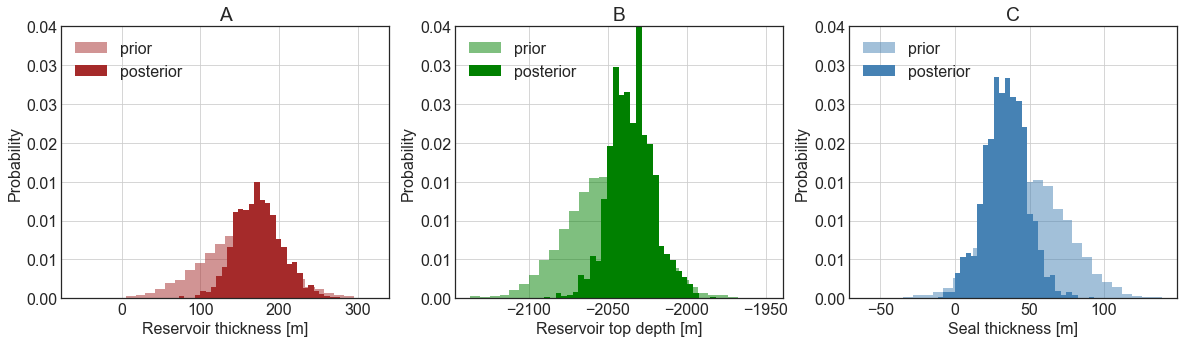
\includegraphics[width=1\textwidth]{Figures/3_parameters.png}
		\caption{Probability distributions for the three parameters used for modeling reservoir score.}\label{fig:3_parameters}
	\end{figure}
	
	\subsection{Two parameters scoring}
	
	Assuming that reservoir thickness is a simplified indicator for the extractable oil or gas and thus value in place, a gain in score can be correlated with increase in thickness. Here, two score points are assigned to one meter of thickness. Increasing costs of drilling are indicated by increasing depth of the reservoir top. Consequently, one negative score point is ascribed to every meter in depth. Samples from the probability distributions of these two parameters are drawn to model the true score of the reservoir (depth scores are subtracted from reservoir thickness scores). For the data used here, it can be seen in Figure \ref{fig:score_results1}-A, that the results of modeling with only these two parameters, are represented by an approximately normal distribution. The score is negative in about 17\% of the cases. Mean and median are about the same.
	
	\subsection{Three parameters scoring}
	
	Next, influence by the third parameter seal thickness is included. Score points are not added or subtracted by this parameter directly. Instead, a threshold for seal reliability is defined beforehand. Here it is set at 20 m thickness. If the seal thickness falls below this threshold, it is assumed that the seal fails completely and thus all the potential value (positive score) of the reservoir is lost, while costs of depth (negative score) remain. Thus, a condition to check whether the seal is reliable is now included in the model. Results are visualized in Figure \ref{fig:score_results1}-B. The main distribution is not changed significantly, except for a striking peak of probability at the possibility of a score of -2000. Furthermore, mean and median have been shifted to lower values and are now found further apart.
	
	\begin{figure}[h]
		\centering
		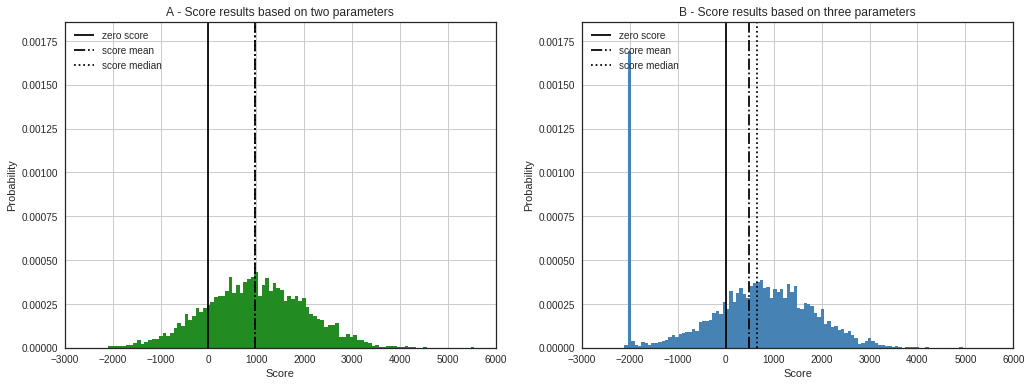
\includegraphics[width=1\textwidth]{Figures/score_results1.png}
		\caption{Posterior probability distributions from modeling scores using two (A) and three parameters (B).}\label{fig:score_results1}
	\end{figure}
	
	\section{Designing a case-specific loss function}
	
	Now that a distribution of reservoir score probabilities has been modeled, a loss function for estimation of the true score value can be developed.
	
	\subsection{Testing standard loss functions}
	
	Some standard loss function were presented in chapter \ref{sec:loss}. For this case, the absolute-error loss and the squared-error loss function were considered as starting points, to design a more case-specific loss function. 	
	Calculating the expected loss for estimates ranging from -3000 to 6000 based on these two standard loss function results in the graphs depicted in Figure \ref{fig:abs_sqr_LF}. It can be observed that the median of the distribution coincides with the minimum of the absolute-error and the mean with the minimum of the squared-error expected loss.
	
	\begin{figure}[h]
		\centering
		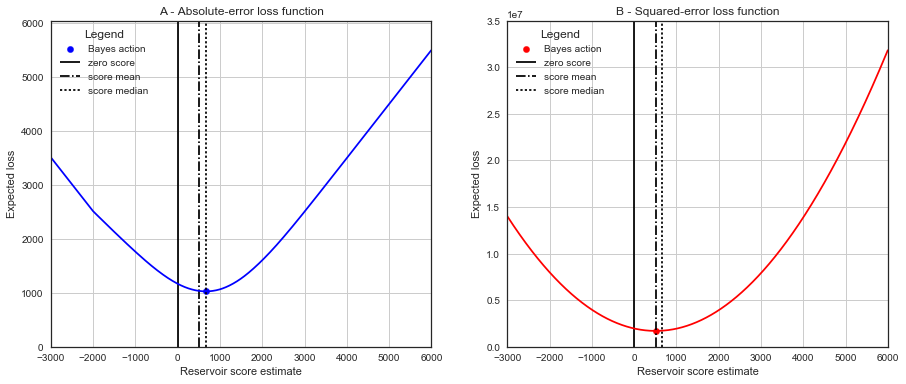
\includegraphics[width=1\textwidth]{Figures/abs_sqr_LF.png}
		\caption{Expected loss based on the standard absolute-error (A) and squared-error (B) loss functions applied on the probability distribution resulting from \ref{sec:scoring} and for estimates ranging from -3000 to 6000.}\label{fig:abs_sqr_LF}
	\end{figure}
	
	\subsection{Adaptions for loss function customization}
	
	These standard loss functions provide objectively good estimators minimizing expected loss. Due to their symmetric properties, both will always give the median or mean of the underlying distribution as minimizing estimator respectively. However, assigning an economic notion to our model and assuming the case of an actor or decision maker in any field, naturally necessitates the consideration of preferences, interests and the overall subjective perspective such an individual or for example a company might have. Further constraints, properties and factors can also be specific to the field, industry or generally to the problem at hand. Consequently, the design of a more specific non-standard and possibly asymmetric loss function might be required, so that an adapted Bayesian estimator can be found. One that includes subjective aspects and difference in weighting of particular gains or losses, arising from an actor's inherent preferences and the environment in which the actor has to estimate or make a decision. In the face of several uncertain parameters, a perfectly true estimate is virtually unattainable. However, an attempt can be made, to design a customized loss function that returns a Bayesian estimator involving the least bad consequences for an individual in a specific environment. Regarding the petroleum system case modeled above, such an attempt is made and explained step by step in the following. 
	
	For the purpose of estimation, it makes sense that one of the standard loss functions is chosen as a basis and a customized loss function is developed from there. The absolute-error loss seems most appropriate for this case of petroleum reservoir quality estimation. As stated above, the reservoir score is an abstract and simplified way to reflect a value contained in the reservoir. Ideally, an actor would like to know the exact true score, so that investments or resources can be allocated appropriately, in order to acquire economic gains. This allocation is the decision to be made or action to be taken. Deviations from the unknown true score in the form of over- and underestimation bring about an error and loss accordingly. In this case, there is no reason for loss to increase exponentially with distance from the true value. It is assumed that investments increase linearly with linear growth in the value of the resource. For this reason, the absolute-error loss function is favored over the squared-error loss function in this case. Some customization steps are taken below, based on mostly logical case-specific assumptions.
	
	\begin{enumerate}
		\item Step I: The standard symmetrical absolute-error loss function is chosen as a starting point for further customization steps:
		
		\begin{equation}
		L(\theta,\hat{\theta}) = |\theta - \hat{\theta}|
		\end{equation}  
		
		\item Step II: Considering the development of a petroleum reservoir, it can be assumed that over-investing is worse than under-investing. Overestimating the size of a reservoir might for example lead to the installation of equipment or facilites that are actually redundant or unnecessary. This would come with additional unrecoverable expenditures. Consequences from underestimating, however, may presumably be easier to resolve. Additional equipment can often be installed later on. Hence, overestimation is weighted stronger in our loss function by multiplying the error with an overestimation factor \textit{a} (= 1.25):
		
		\begin{equation}\label{eq:LF_II}
		L(\theta,\hat{\theta}) = |(\theta-\hat{\theta})|*a
		\end{equation}
		
		\item Step III: The worst case for any project would be that its development is set into motion, expecting a gain, only to discover later that the value in the reservoir does not cover the costs of realizing the project, resulting in an overall loss. A petroleum system might also turn out to be a complete failure, containing no value at all, although the actor's estimate indicated the opposite. Here, this is referred to as a worst case or fatal overestimation. A positive score is estimated, but the true score is zero or negative. This is worse than the "normal" non-fatal overestimation, where both values are positive and a net gain is still achieved, which is only smaller then the best possible gain of expecting the true score. Fatal overestimation is included in the loss function by using another weighting factor \textit{b} (= 2) that replaces \textit{a}:
		
		\begin{equation}\label{eq:LF_III}
		L(\theta,\hat{\theta}) = |(\theta-\hat{\theta})|*b
		\end{equation}
		
		(In other words: Worst case or fatal overestimation is twice as bad as simple underestimation.)
		
		\item Step IV: A worst case or fatal underestimation can also be derived from the idea of estimating a zero or negative score, when the true score is actually positive. This is assumed to be worse than non-fatal overestimation, but clearly better than fatal overestimation. No already owned resources are wasted, it is only the potential value that is lost, i.e. opportunity costs that arise from completely discarding a reservoir with a potential gain equal to the positive true score. Fatal underestimation is weighted using a third factor \textit{c}:
				
		\begin{equation}\label{eq:LF_IV}
		L(\theta,\hat{\theta}) = |(\theta-\hat{\theta})|*c
		\end{equation}
		
	\end{enumerate}
	
	Combining these adaption steps and the conditions defined in them, results in the following customized loss function:
	
	\begin{equation}\label{eq:LF_final}
	L(\theta,\hat{\theta}) =
	\begin{cases}
	|\theta - \hat{\theta}|, & \text{for } 0<\hat{\theta}<\theta  \\
	|\theta-\hat{\theta}|*a, & \text{for } 0<\theta<\hat{\theta} \\
	|\theta-\hat{\theta}|*b, & \text{for } \theta\leq0<\hat{\theta} \\
	|\theta-\hat{\theta}|*c, & \text{for } \hat{\theta}\leq0<\theta 
	\end{cases},
	\text{ with } a,b,c \in \mathbb{Q}
	\end{equation}
	  
	Realizations of the four adaption steps are depicted in the plots in Figure \ref{fig:LF_4steps}. It is important to note that the weighting factors defined above can take basically any numerical values but should be chosen in a way that they appropriately represent the framework conditions of the problem. Here, for example, it is assumed that normal overestimation is 25\% (\textit{a} = 1.25), fatal overestimation 100\% (\textit{b} = 2) and fatal underestimation 50\% (\textit{c} = 1.5) worse than normal underestimation. 
	
	\begin{figure}[h]
		\centering
		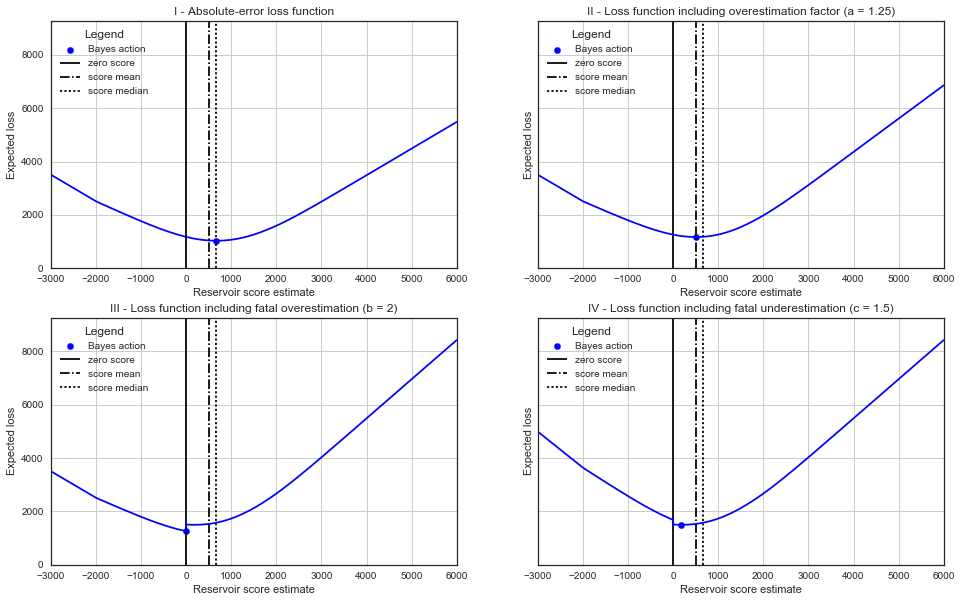
\includegraphics[width=1\textwidth]{Figures/LF_4steps.png}
		\caption{The single steps of customizing the loss function are depicted in plots I - IV.}\label{fig:LF_4steps}
	\end{figure}
	
	In Figure \ref{fig:LF_4steps} it can be observed, that assigning a stronger weight on overestimation (plot II) steepens the curve on the right hand side and shifts the minimum to the left, i.e. to a lower estimate. Using \textit{a} = 1.25, the Bayes action changes from the median, to a value close to the mean of the distribution. The shift and steepening are significantly reinforced by the introduction of fatal overestimation (plot III). With \textit{b} = 2, the Bayes action drops to the zero score estimate. It can also be noted, that by defining a condition dependent on the algebraic sign of the values, according to which only losses for positive estimates are multiplied by \textit{b}, a distinct jump appears at the zero score boundary. Due to a similar condition, the same effect is observed on the negative side of estimate values, where the curve has also been steepened, after including fatal underestimation (plot IV). This comes with a shift of the minimum towards positive values. It is also to be noted that with every customization step, the overall expected loss is increased.
	
	\begin{figure}[h]
		\centering
		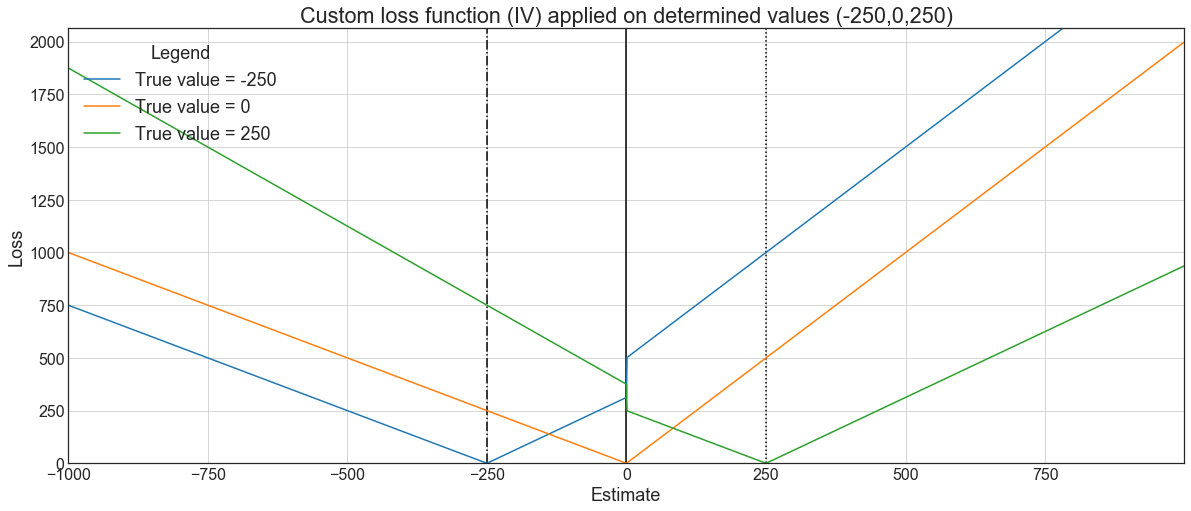
\includegraphics[width=1\textwidth]{Figures/LF4_det_values.png}
		\caption{Loss based on the customized loss function (IV) for determined true scores of -750, 0 and 750.}\label{fig:LF4_det_values}
	\end{figure}
	
	The implementation of this customized loss function (IV) using single determined values for the true score is plotted in Figure \ref{fig:LF4_det_values}. This helps to clarify the way real losses result for each guess, relative to given true score values. The expected loss is acquired by arithmetically averaging such loss realizations based on the true score probability distribution by using formula \ref{eq:ExpectedLoss2}.
	
	It has to be emphasized that this is just one possible proposal for loss function customization. There exists not one perfect design for such a case. Slight to strong changes can already be implemented by simply varying the values of the weighting factors \textit{a, b} and \textit{c}. Fundamentally different loss functions can also be based on a significantly different mathematical structure. Loss functions are customized regarding the problem environment and according to the to the subjective needs and objectives of an actor. Thus, they are mostly defined by the actor expressing his perspective. Changes in the individual's perception and viewpoint might lead to further customization needs even later on. (Especially considering individual persons as actors, psychological aspects may play a significant role.)
	
	(Estimate or prediction? True value only known if a "yes"-action (development) is taken.)
	
	\subsection{Including different risk-affinities in the loss function}
	
	One can assume that several actors in one sector or decision environment may have the same general loss function, but different affinities concerning risks. This might be based for example on the different psychological factors or economic philosophies followed by companies. It might also be based on budgets and options such actors have available. An intuitive example is the comparison of a small and a large company. A certain false estimate or error might have a significantly stronger impact on a company which has a a generally lower market share and only few projects, than on a larger company which might possess a higher financial flexibility and for which one project is only one of many development options in a portfolio.
	
	In the following, the loss function is further adapted to consider different risk-affinities of several actors. Representing risk behavior in a loss function can also be done in different ways and regarding different types of risks. Here, bidding lower is considered the cautious, risk-averse option, as smaller losses can be expected from underestimating. Guessing higher is deemed riskier. Losses from overestimation are greater. However, bidding correctly on a higher value, will also return a greater gain. It is assumed that risk-friendly actors care less about fatal underestimation, i.e. they will rather develop a project than discard it. In the loss function, risk is simply included using a risk factor \textit{r} which alters the weighting factors \textit{a, b} and \textit{c} respectively:
	
	\begin{equation}\label{eq:LFR_final}
	L(\theta,\hat{\theta}) =
	\begin{cases}
	|\theta - \hat{\theta}|, & \text{for } 0<\hat{\theta}<\theta  \\
	|\theta-\hat{\theta}|*(a*r), & \text{for } 0<\theta<\hat{\theta} \\
	|\theta-\hat{\theta}|*(b*r), & \text{for } \theta\leq0<\hat{\theta} \\
	|\theta-\hat{\theta}|*(c*(r^{-0.5})), & \text{for } \hat{\theta}\leq0<\theta 
	\end{cases},
	\text{ with } a,b,c,r \in \mathbb{Q}
	\end{equation}
	
	According to this, for \textit{r} = 1 the risk-neutral loss function is returned, since \textit{a, b} and \textit{c} are not altered. For \textit{r} $<$ 1, the weight on overestimating is reduced and increased for fatal underestimation. This represents a more risk-friendly actor that is willing to bid on a higher estimate to attain a greater gain. For \textit{r} $>$ 1, the overestimation weight is increased, the underestimation weight decreased in the loss function and respectively more risk-averse actors are prompted to bid on lower estimates. 
	
	The factor \textit{r} can take basically any positive values. However, since risk-neutrality is expressed by\textit{r} = 1, values 0 $<$ \textit{r} $<$ 2 are considered to be the most appropriate choices to represent both sides of risk-affinity equally. 
	
	Implementing it as a factor \textit{r} leads to different steepnesses of the plotted curves depicting loss and expected loss. The effect on the latter is visualized in Figure \ref{fig:LFR}, where 0.5, 0.75, 1, 1.25 and 1.5 were chosen as values for \textit{r}. 	
	It can be observed that the minima for expected loss, i.e. the Bayesian estimators for differently risk-affine actors, are located at different estimates. Mean and median are clearly surpassed by the best estimate of the most risk-friendly actor (\textit{r} = 0.5), while for the most risk-averse actors (\textit{r} 0.5 and \textit{r} = 0.75), the Bayes action equals a zero score estimate (and thus the decision to take on action). In Figure \ref{fig:LFR} it can also be recognized that the expected loss is generally lower for risk-friendlier actors (on the side of positive estimates).
	
	\begin{figure}[h]
		\centering
		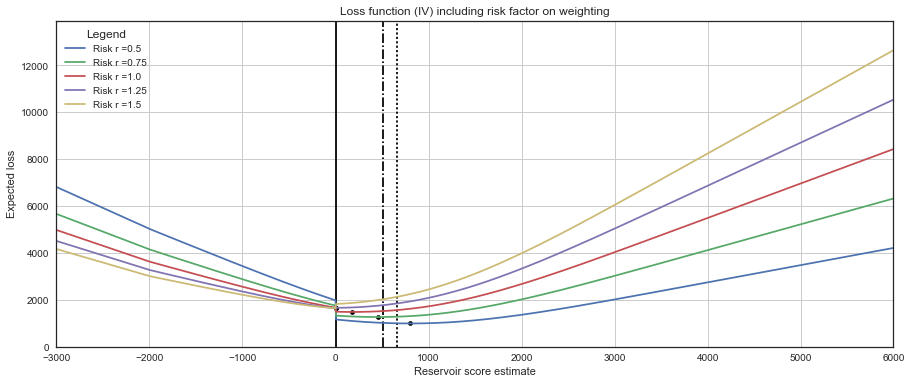
\includegraphics[width=1\textwidth]{Figures/LFR.png}
		\caption{Plotting of expected loss realizations after including the risk factor r in the loss function (IV) for actors with risk-affinities ranging from risk-averse (r = 0.5 and 0.75), over risk-neutral (r = 1), to risk-friendly (r = 1.25 and r = 1.5).}\label{fig:LFR} 
	\end{figure}
	
	\section{Updating the model with additional information in the form of thickness likelihoods}
	
	\citet{delaVarga2016} made use of Bayesian inference to reduce the uncertainty in this type of one-dimensional model. The same is conducted here in the following.
	
	The probability distributions for the location of the layer boundaries are treated as priors. Now it is assumed that new observations have been made, providing additional information on the likelihoods of the thicknesses of the two layers. Likelihood functions for reservoir and seal thicknesses are introduced in the form of normal distributions, defined by means and standard deviations. These parameters vary according to nature of the observations made. Using the principle of Bayesian inference as explained in \ref{cha:met}, the model is updated and new posterior distributions for our true reservoir score are attained.
	
	- VOI Quantification ???
	
	Different examples with different sets of likelihoods are conducted in the following, so that various possible results can be compared. Each take the layer boundaries defined in  \ref{sec:1D_construction} as priors and use Bayesian inference with data defined below for each example.
	
	\subsection{Updating example I (moderate reinforcement)- Seal: mean = 25~m, std = 20~m - Reservoir: mean = 180~m, std = 60~m}
	
	\begin{figure}[h]
		\centering
		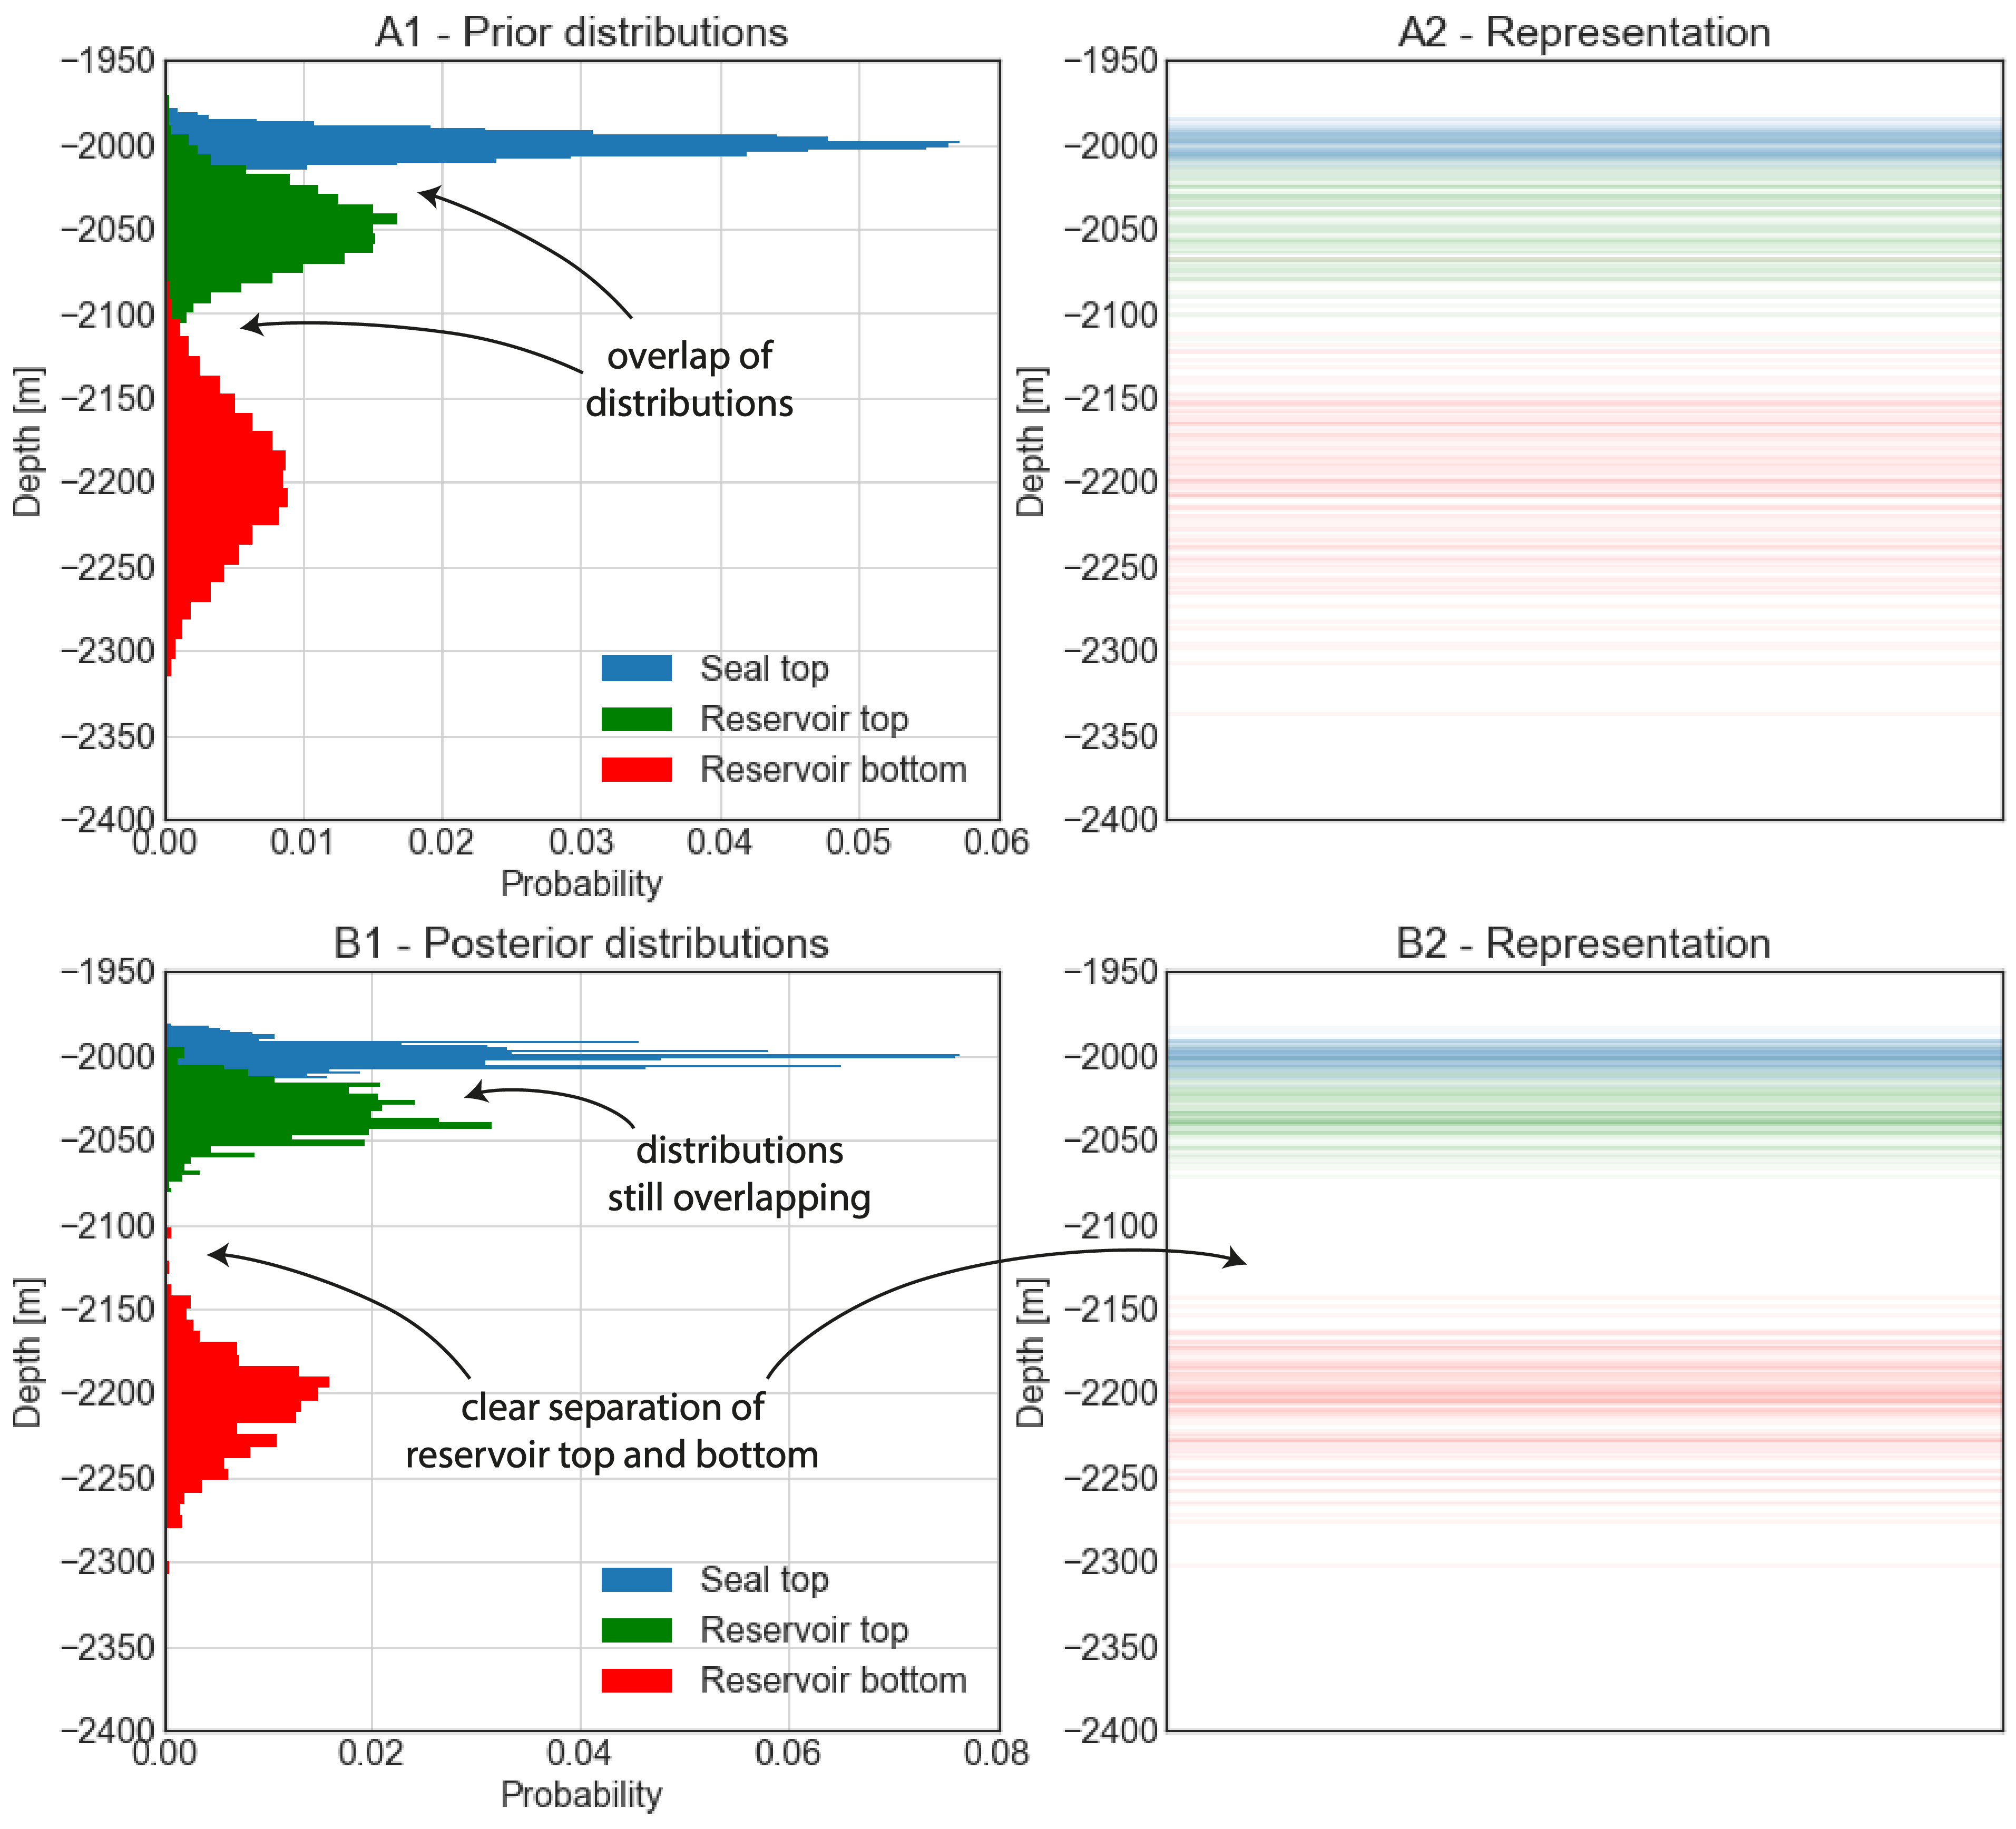
\includegraphics[width=1\textwidth]{Figures/update_moderate1.png}
		\caption{...}\label{fig:update_moderate1} 
	\end{figure}
	
	In this first case, a normal distribution with a mean of 25~m and a standard deviation of 20~m is chosen to reflect the likelihood of the seal thickness. For the reservoir, a normal distribution with a mean of 180~m and a standard deviation of 60~m is chosen. Using these likelihoods to update the one-dimensional model, the uncertainty in the posterior probability distributions for the positions of layer boundaries in depth is reduced (see Figure \ref{fig:update_moderate1}).
		
	Modeling the reservoir score is conducted as above, now based on these new distributions. In Figure \ref{fig:update_moderate2} it can be recognized that the bulk of the distribution was shifted to the positive side of scores, while the peak at -~2000 was raised. The probability of scores between -~2000 and 0 decreased significantly, i.e. the true score is most likely either positive or -~2000 if it is negative.
	
	\begin{figure}[h]
		\centering
		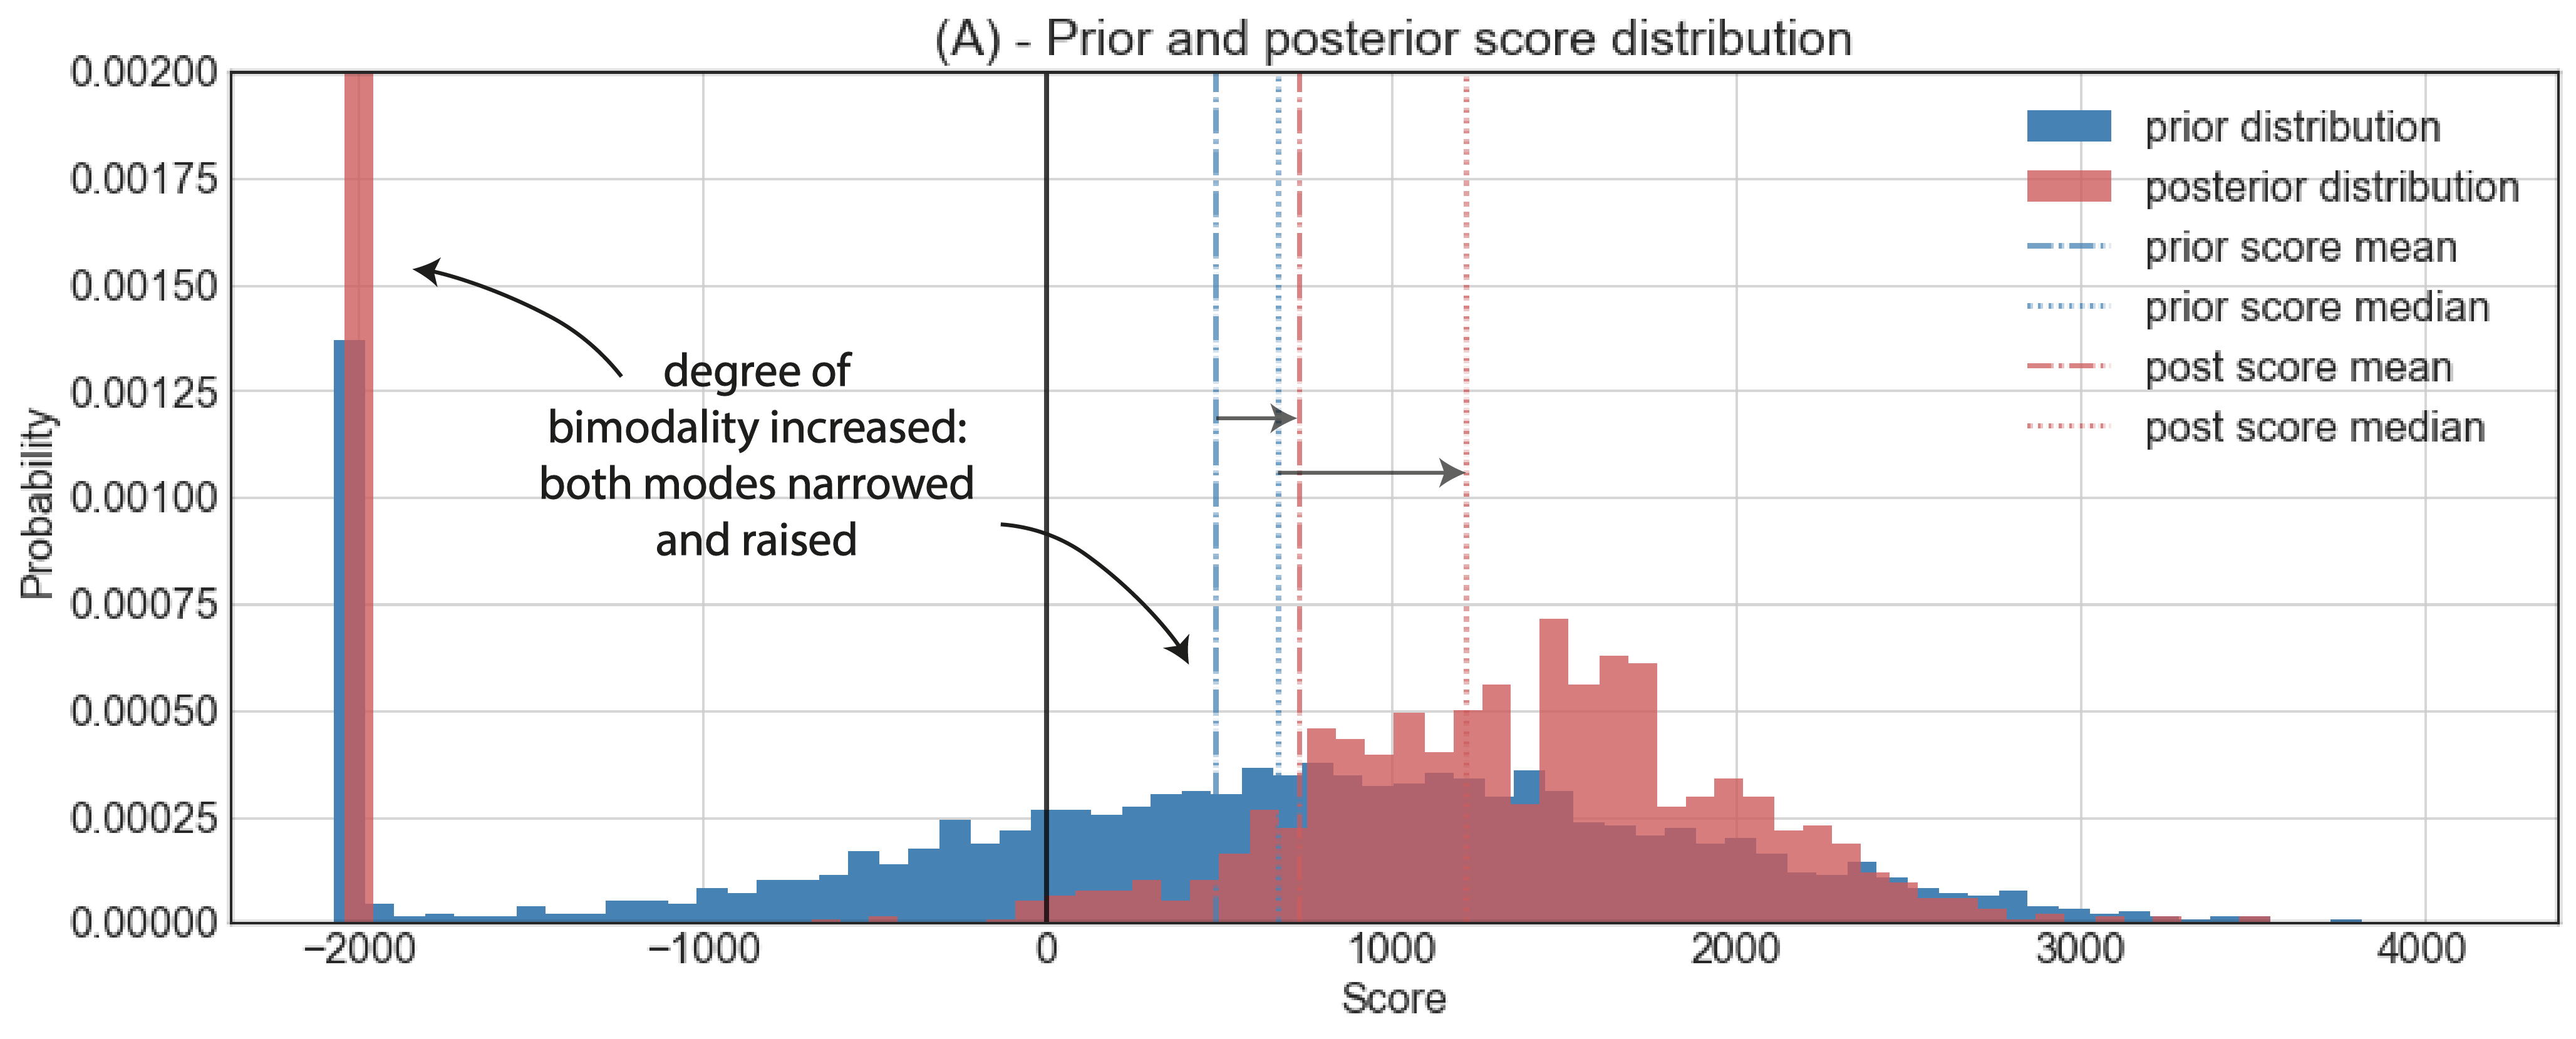
\includegraphics[width=1\textwidth]{Figures/update_moderate2.png}
		\caption{...}\label{fig:update_moderate2} 
	\end{figure}
	
	\begin{figure}[h]
		\centering
		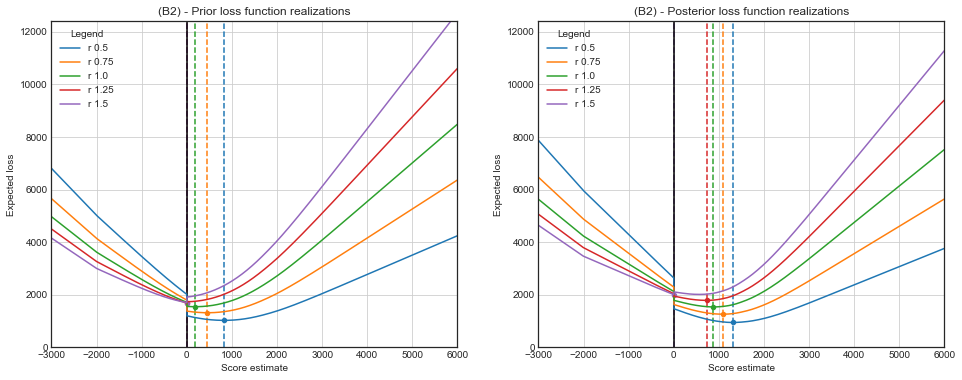
\includegraphics[width=1\textwidth]{Figures/update_moderate3.png}
		\caption{...}\label{fig:update_moderate3} 
	\end{figure}
	
	The customized loss function (IV) is now applied on this updated distribution of the reservoir score. This is visualized in Figure \ref{fig:update_moderate3} in which the expected losses are compared before (B1 )and after (B2) uncertainty reduction. It is observable, that by adding information about layer thickness likelihoods, Bayes actions are shifted relative to the nature of the information. In this case, the added data generally reinforces the likelihoods of the reservoir to be significantly thick. Information on the seal, however, based on a normal distribution around 25~m thickness, leaves uncertainty about the reliability of the seal, as the safety threshold is defined as 20~m. 
	
	\begin{table}
		\centering
		\begin{tabular}[c]{| l | l | l |}
			\hline
			Risk factor \textit{r} & Shift in Bayes action & Change in expected loss \\ \hline
			0.50 & +~553.67 & -~105.49 \\ 
			0.75 & +~673.40 & -~81.67  \\ 
			1.00 & +~750.05 & -~33.56 \\ 
			1.25 & +~713.19 & +~75.71 \\ 
			1.50 & +~0.00 & +~282.64  \\ 
			\hline
		\end{tabular}
		\caption{Bla}
		\label{tab:update_moderate_tab}
	\end{table}
	
	Increased certainty about the reservoir thickness is sufficient to shift Bayes actions to higher estimates for all actors, but the most risk-averse one. These shifts are quantified in Table \ref{tab:update_moderate_tab}. According to these numbers, the risk-neutral actor's estimate is increased the most. Expected losses decreased for the risk-neutral and the two risk-friendlier individuals. It is clear that the expected loss was reduced the most for the risk-friendliest actor and it increased most significantly for the most risk-averse actor.
	
	\subsection{Updating example II (reliable seal) - Seal: mean = 50 m, std = 20 m - Reservoir: mean = 180 m, std = 60 m}
	
	In this second case, the reservoir thickness likelihood is defined in the same way as before. For the seal, a mean of 50~m with a standard deviation of 20~m is chosen, favoring the likelihood of a reliable seal relative to the threshold of 20~m thickness. This results in the score distribution depicted in \ref{fig:update_goodseal2}. The bulk of the distribution is narrowed on the positive side of estimates. Mean and median are clearly shifted to higher values as well. The "seal failure" peak at -~2000 is significantly. decreased.
	
	\begin{figure}[h]
		\centering
		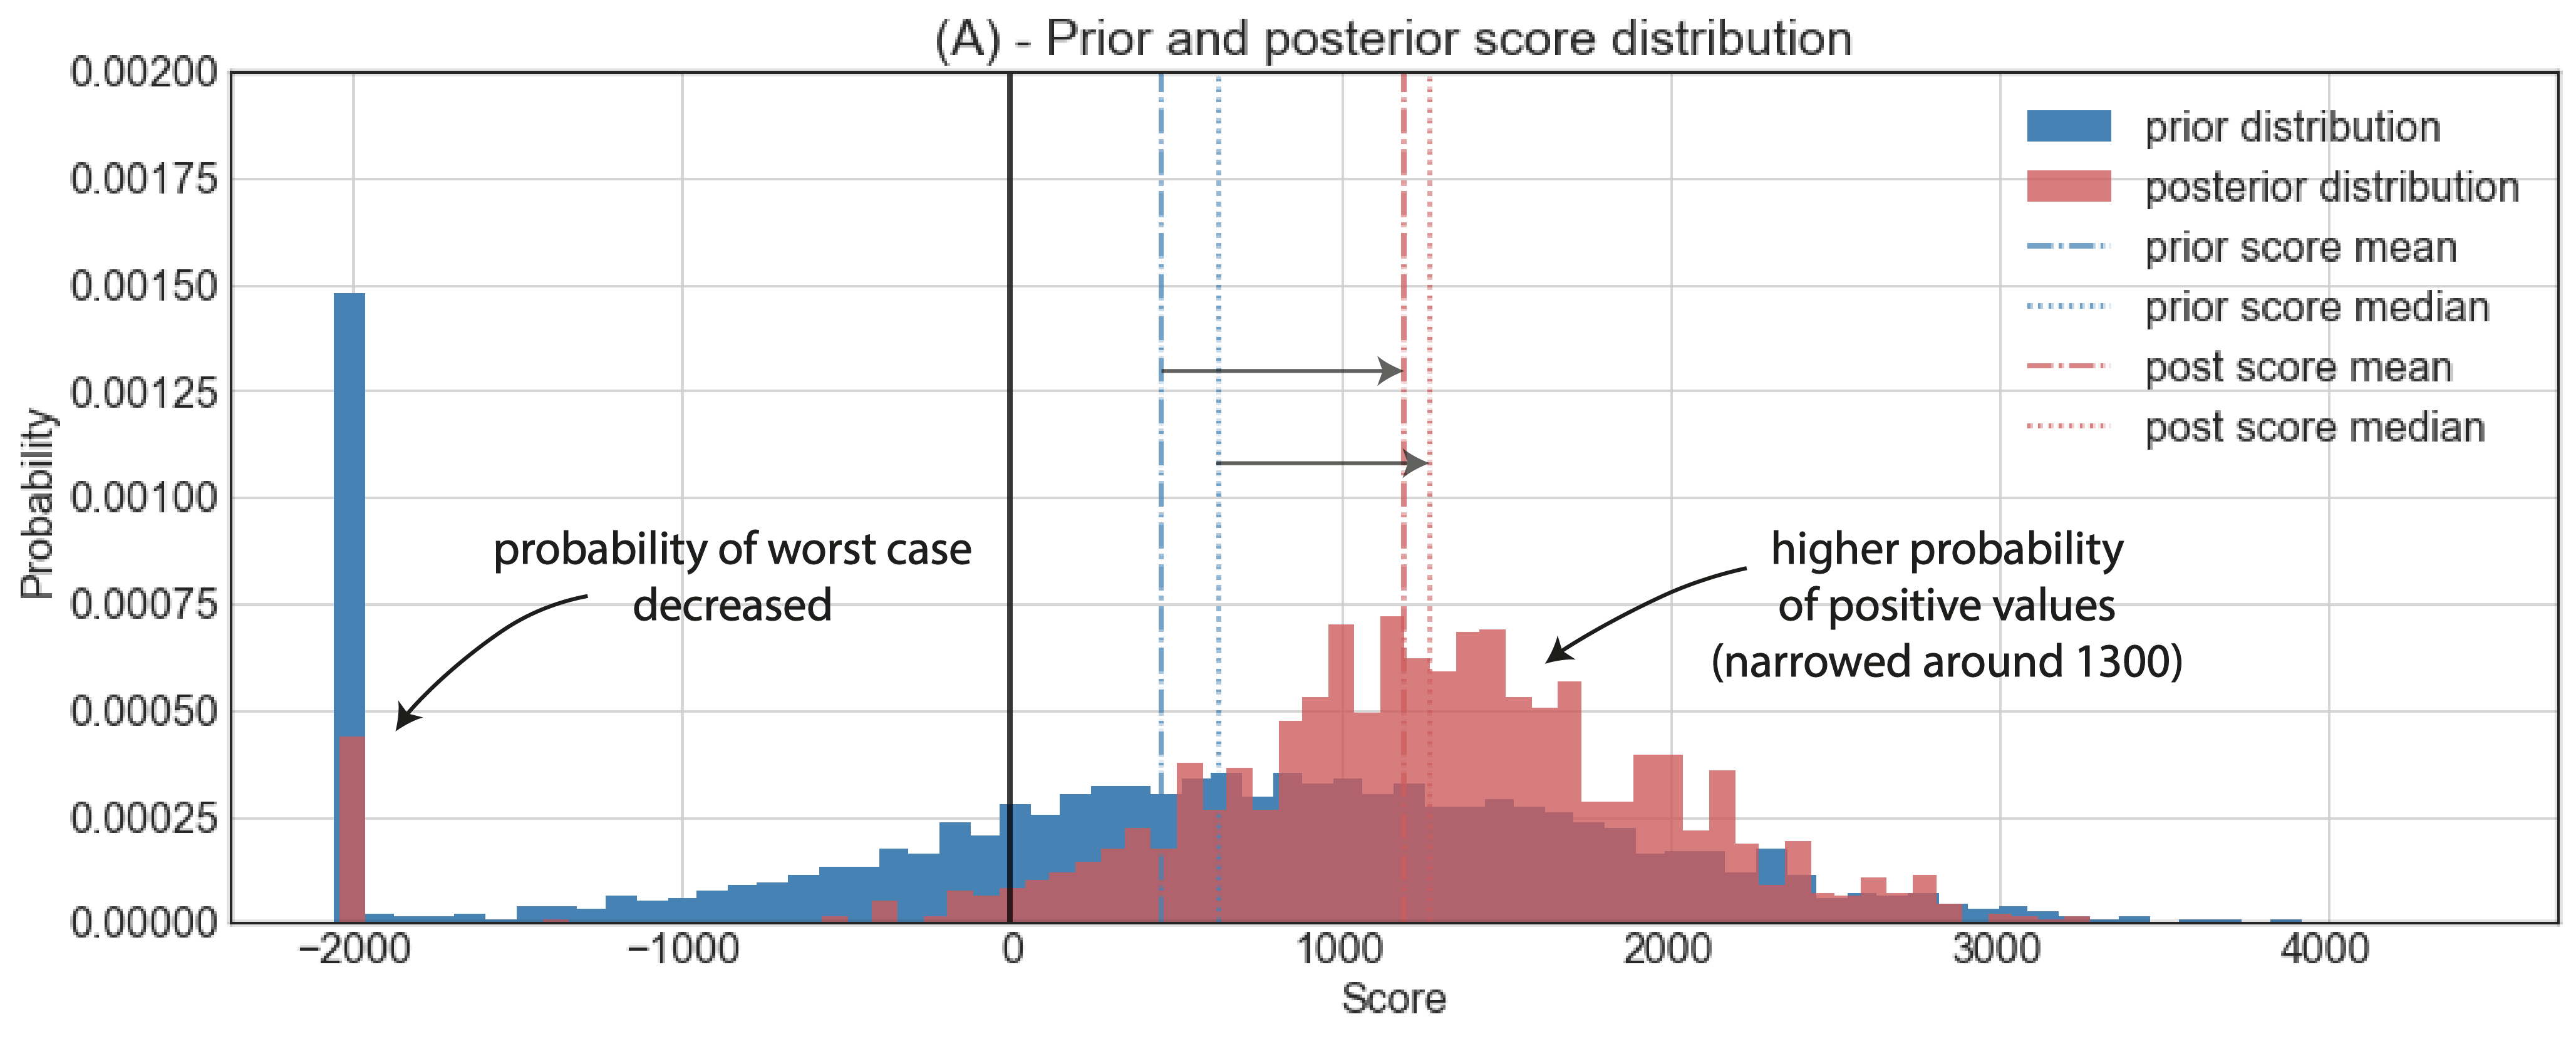
\includegraphics[width=1\textwidth]{Figures/update_goodseal2.png}
		\caption{...}\label{fig:update_goodseal2} 
	\end{figure}
	
	Applying the loss function on this new score distribution results in the realizations of expected loss illustrated in \ref{fig:update_goodseal3}. Bayes actions are shifted clearly to higher estimates and expected losses of these minima are significantly reduced for all actors. This is quantified in \ref{tab:update_goodseal_tab}. According to these values, the risk-neutral to risk-averse individuals seem to profit the most.
	
	\begin{figure}[h]
		\centering
		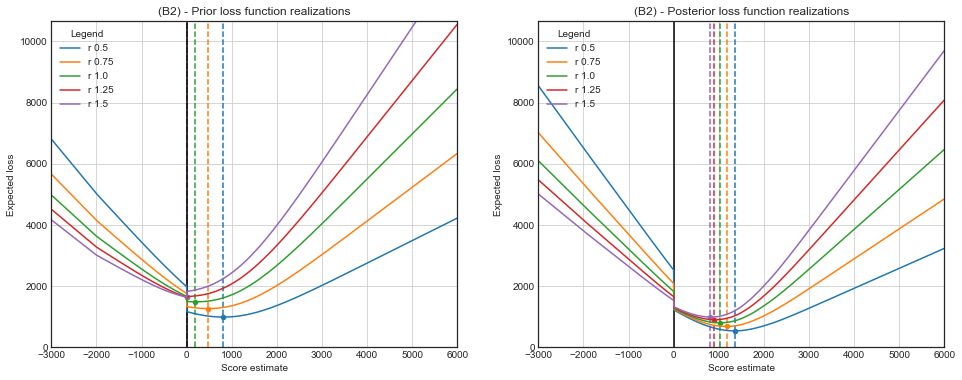
\includegraphics[width=1\textwidth]{Figures/update_goodseal3.png}
		\caption{...}\label{fig:update_goodseal3} 
	\end{figure}
	
	\begin{table}
		\centering
		\begin{tabular}[c]{| l | l | l |}
			\hline
			Risk factor \textit{r} & Shift in Bayes action & Change in expected loss \\ \hline
			0.50 & +~522.95 & -~436.26 \\ 
			0.75 & +~697.73 & -~551.92  \\ 
			1.00 & +~855.57 & -~631.92 \\ 
			1.25 & +~912.43 & -~647.10 \\ 
			1.50 & +~819.26 & -~545.96  \\ 
			\hline
		\end{tabular}
		\caption{Bla}
		\label{tab:update_goodseal_tab}
	\end{table}
	
	\subsection{Updating example III (safe seal, but reservoir under average) - Seal: mean = 70 m, std = 10 m - Reservoir: mean = 100 m, std = 40 m}
	
	In this third example, seal safety is ensured by using a mean of 70~m with a standard deviation of 10~m for the seal thickness likelihood. However, the new observations are assumed to provide information about the reservoir that makes it likely to be thinner as expected. Reservoir thickness likelihood is assigned a mean of 100~m and a standard deviation of 10~m. 
	
	The subsequent score distribution is depicted in \ref{fig:update_smallres2}. It can be seen that while the whole distribution is narrowed, it also is shifted to the left, to lower and negative estimates. Mean and median are almost the same. As seal reliability is practically guaranteed, the peak at -~2000~m vanishes. 
	
	Based on this probability distribution of the reservoir score, Bayes actions are shifted to lower estimates for all actors (\ref{fig:update_smallres3}). In fact, also but the most risk-friendly individual (\textit{r} = 0.5) find their Bayesian estimator to be zero now, i.e. project development is deemed to be too risky to them. Furthermore, the spread of expected loss values around the minima for all actors is diminished (the expected loss values of the Bayes actions are now much closer to each other).
	
	Quantified changes in the position and the values of the Bayes actions are comparable to the results in example II (there is no shift for risk-averse actors, as they already found their best estimates to be zero). Most notable is the large reduction of expected loss in general (see \ref{tab:update_smallres_tab}).	
	
	\begin{figure}[h]
			\centering
			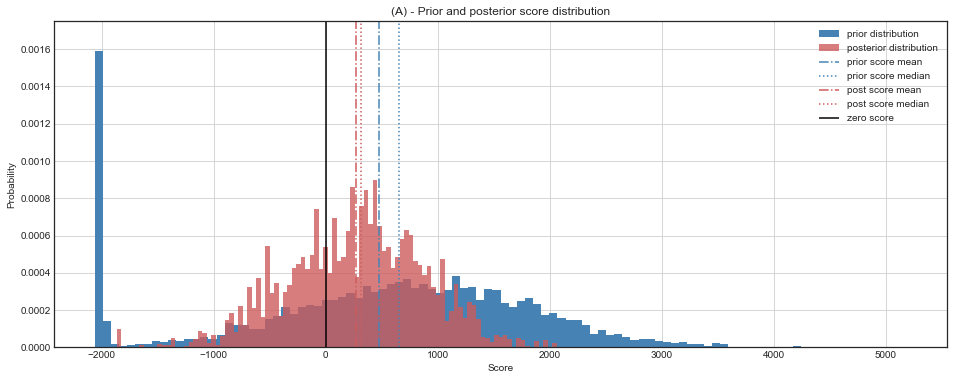
\includegraphics[width=1\textwidth]{Figures/update_smallres2.png}
			\caption{...}\label{fig:update_smallres2} 
	\end{figure}
	
	\begin{figure}[h]
				\centering
				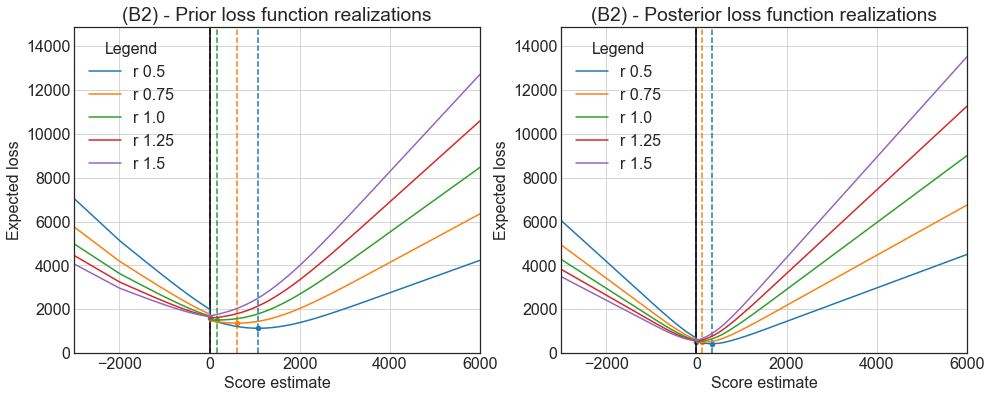
\includegraphics[width=1\textwidth]{Figures/update_smallres3.png}
				\caption{...}\label{fig:update_smallres3} 
	\end{figure}
			
	\begin{table}
		\centering
		\begin{tabular}[c]{| l | l | l |}
			\hline
			Risk factor \textit{r} & Shift in Bayes action & Change in expected loss \\ \hline
			0.50 & -~498.98 & -~538.08 \\ 
			0.75 & -~346.16 & -~717.83  \\ 
			1.00 & -~176.13 & -~872.02 \\ 
			1.25 & -~0.00 & -~946.04 \\ 
			1.50 & -~0.00 & -~951.57  \\ 
			\hline
		\end{tabular}
		\caption{Bla}
		\label{tab:update_smallres_tab}
	\end{table}
		
	\section{General case results}